\documentclass{article} % For LaTeX2e
\usepackage{iclr2027_conference,times}

% Optional math commands from https://github.com/goodfeli/dlbook_notation.
%%%%% NEW MATH DEFINITIONS %%%%%

\usepackage{amsmath,amsfonts,bm}

% Mark sections of captions for referring to divisions of figures
\newcommand{\figleft}{{\em (Left)}}
\newcommand{\figcenter}{{\em (Center)}}
\newcommand{\figright}{{\em (Right)}}
\newcommand{\figtop}{{\em (Top)}}
\newcommand{\figbottom}{{\em (Bottom)}}
\newcommand{\captiona}{{\em (a)}}
\newcommand{\captionb}{{\em (b)}}
\newcommand{\captionc}{{\em (c)}}
\newcommand{\captiond}{{\em (d)}}

% Highlight a newly defined term
\newcommand{\newterm}[1]{{\bf #1}}


% Figure reference, lower-case.
\def\figref#1{figure~\ref{#1}}
% Figure reference, capital. For start of sentence
\def\Figref#1{Figure~\ref{#1}}
\def\twofigref#1#2{figures \ref{#1} and \ref{#2}}
\def\quadfigref#1#2#3#4{figures \ref{#1}, \ref{#2}, \ref{#3} and \ref{#4}}
% Section reference, lower-case.
\def\secref#1{section~\ref{#1}}
% Section reference, capital.
\def\Secref#1{Section~\ref{#1}}
% Reference to two sections.
\def\twosecrefs#1#2{sections \ref{#1} and \ref{#2}}
% Reference to three sections.
\def\secrefs#1#2#3{sections \ref{#1}, \ref{#2} and \ref{#3}}
% Reference to an equation, lower-case.
\def\eqref#1{equation~\ref{#1}}
% Reference to an equation, upper case
\def\Eqref#1{Equation~\ref{#1}}
% A raw reference to an equation---avoid using if possible
\def\plaineqref#1{\ref{#1}}
% Reference to a chapter, lower-case.
\def\chapref#1{chapter~\ref{#1}}
% Reference to an equation, upper case.
\def\Chapref#1{Chapter~\ref{#1}}
% Reference to a range of chapters
\def\rangechapref#1#2{chapters\ref{#1}--\ref{#2}}
% Reference to an algorithm, lower-case.
\def\algref#1{algorithm~\ref{#1}}
% Reference to an algorithm, upper case.
\def\Algref#1{Algorithm~\ref{#1}}
\def\twoalgref#1#2{algorithms \ref{#1} and \ref{#2}}
\def\Twoalgref#1#2{Algorithms \ref{#1} and \ref{#2}}
% Reference to a part, lower case
\def\partref#1{part~\ref{#1}}
% Reference to a part, upper case
\def\Partref#1{Part~\ref{#1}}
\def\twopartref#1#2{parts \ref{#1} and \ref{#2}}

\def\ceil#1{\lceil #1 \rceil}
\def\floor#1{\lfloor #1 \rfloor}
\def\1{\bm{1}}
\newcommand{\train}{\mathcal{D}}
\newcommand{\valid}{\mathcal{D_{\mathrm{valid}}}}
\newcommand{\test}{\mathcal{D_{\mathrm{test}}}}

\def\eps{{\epsilon}}


% Random variables
\def\reta{{\textnormal{$\eta$}}}
\def\ra{{\textnormal{a}}}
\def\rb{{\textnormal{b}}}
\def\rc{{\textnormal{c}}}
\def\rd{{\textnormal{d}}}
\def\re{{\textnormal{e}}}
\def\rf{{\textnormal{f}}}
\def\rg{{\textnormal{g}}}
\def\rh{{\textnormal{h}}}
\def\ri{{\textnormal{i}}}
\def\rj{{\textnormal{j}}}
\def\rk{{\textnormal{k}}}
\def\rl{{\textnormal{l}}}
% rm is already a command, just don't name any random variables m
\def\rn{{\textnormal{n}}}
\def\ro{{\textnormal{o}}}
\def\rp{{\textnormal{p}}}
\def\rq{{\textnormal{q}}}
\def\rr{{\textnormal{r}}}
\def\rs{{\textnormal{s}}}
\def\rt{{\textnormal{t}}}
\def\ru{{\textnormal{u}}}
\def\rv{{\textnormal{v}}}
\def\rw{{\textnormal{w}}}
\def\rx{{\textnormal{x}}}
\def\ry{{\textnormal{y}}}
\def\rz{{\textnormal{z}}}

% Random vectors
\def\rvepsilon{{\mathbf{\epsilon}}}
\def\rvtheta{{\mathbf{\theta}}}
\def\rva{{\mathbf{a}}}
\def\rvb{{\mathbf{b}}}
\def\rvc{{\mathbf{c}}}
\def\rvd{{\mathbf{d}}}
\def\rve{{\mathbf{e}}}
\def\rvf{{\mathbf{f}}}
\def\rvg{{\mathbf{g}}}
\def\rvh{{\mathbf{h}}}
\def\rvu{{\mathbf{i}}}
\def\rvj{{\mathbf{j}}}
\def\rvk{{\mathbf{k}}}
\def\rvl{{\mathbf{l}}}
\def\rvm{{\mathbf{m}}}
\def\rvn{{\mathbf{n}}}
\def\rvo{{\mathbf{o}}}
\def\rvp{{\mathbf{p}}}
\def\rvq{{\mathbf{q}}}
\def\rvr{{\mathbf{r}}}
\def\rvs{{\mathbf{s}}}
\def\rvt{{\mathbf{t}}}
\def\rvu{{\mathbf{u}}}
\def\rvv{{\mathbf{v}}}
\def\rvw{{\mathbf{w}}}
\def\rvx{{\mathbf{x}}}
\def\rvy{{\mathbf{y}}}
\def\rvz{{\mathbf{z}}}

% Elements of random vectors
\def\erva{{\textnormal{a}}}
\def\ervb{{\textnormal{b}}}
\def\ervc{{\textnormal{c}}}
\def\ervd{{\textnormal{d}}}
\def\erve{{\textnormal{e}}}
\def\ervf{{\textnormal{f}}}
\def\ervg{{\textnormal{g}}}
\def\ervh{{\textnormal{h}}}
\def\ervi{{\textnormal{i}}}
\def\ervj{{\textnormal{j}}}
\def\ervk{{\textnormal{k}}}
\def\ervl{{\textnormal{l}}}
\def\ervm{{\textnormal{m}}}
\def\ervn{{\textnormal{n}}}
\def\ervo{{\textnormal{o}}}
\def\ervp{{\textnormal{p}}}
\def\ervq{{\textnormal{q}}}
\def\ervr{{\textnormal{r}}}
\def\ervs{{\textnormal{s}}}
\def\ervt{{\textnormal{t}}}
\def\ervu{{\textnormal{u}}}
\def\ervv{{\textnormal{v}}}
\def\ervw{{\textnormal{w}}}
\def\ervx{{\textnormal{x}}}
\def\ervy{{\textnormal{y}}}
\def\ervz{{\textnormal{z}}}

% Random matrices
\def\rmA{{\mathbf{A}}}
\def\rmB{{\mathbf{B}}}
\def\rmC{{\mathbf{C}}}
\def\rmD{{\mathbf{D}}}
\def\rmE{{\mathbf{E}}}
\def\rmF{{\mathbf{F}}}
\def\rmG{{\mathbf{G}}}
\def\rmH{{\mathbf{H}}}
\def\rmI{{\mathbf{I}}}
\def\rmJ{{\mathbf{J}}}
\def\rmK{{\mathbf{K}}}
\def\rmL{{\mathbf{L}}}
\def\rmM{{\mathbf{M}}}
\def\rmN{{\mathbf{N}}}
\def\rmO{{\mathbf{O}}}
\def\rmP{{\mathbf{P}}}
\def\rmQ{{\mathbf{Q}}}
\def\rmR{{\mathbf{R}}}
\def\rmS{{\mathbf{S}}}
\def\rmT{{\mathbf{T}}}
\def\rmU{{\mathbf{U}}}
\def\rmV{{\mathbf{V}}}
\def\rmW{{\mathbf{W}}}
\def\rmX{{\mathbf{X}}}
\def\rmY{{\mathbf{Y}}}
\def\rmZ{{\mathbf{Z}}}

% Elements of random matrices
\def\ermA{{\textnormal{A}}}
\def\ermB{{\textnormal{B}}}
\def\ermC{{\textnormal{C}}}
\def\ermD{{\textnormal{D}}}
\def\ermE{{\textnormal{E}}}
\def\ermF{{\textnormal{F}}}
\def\ermG{{\textnormal{G}}}
\def\ermH{{\textnormal{H}}}
\def\ermI{{\textnormal{I}}}
\def\ermJ{{\textnormal{J}}}
\def\ermK{{\textnormal{K}}}
\def\ermL{{\textnormal{L}}}
\def\ermM{{\textnormal{M}}}
\def\ermN{{\textnormal{N}}}
\def\ermO{{\textnormal{O}}}
\def\ermP{{\textnormal{P}}}
\def\ermQ{{\textnormal{Q}}}
\def\ermR{{\textnormal{R}}}
\def\ermS{{\textnormal{S}}}
\def\ermT{{\textnormal{T}}}
\def\ermU{{\textnormal{U}}}
\def\ermV{{\textnormal{V}}}
\def\ermW{{\textnormal{W}}}
\def\ermX{{\textnormal{X}}}
\def\ermY{{\textnormal{Y}}}
\def\ermZ{{\textnormal{Z}}}

% Vectors
\def\vzero{{\bm{0}}}
\def\vone{{\bm{1}}}
\def\vmu{{\bm{\mu}}}
\def\vtheta{{\bm{\theta}}}
\def\va{{\bm{a}}}
\def\vb{{\bm{b}}}
\def\vc{{\bm{c}}}
\def\vd{{\bm{d}}}
\def\ve{{\bm{e}}}
\def\vf{{\bm{f}}}
\def\vg{{\bm{g}}}
\def\vh{{\bm{h}}}
\def\vi{{\bm{i}}}
\def\vj{{\bm{j}}}
\def\vk{{\bm{k}}}
\def\vl{{\bm{l}}}
\def\vm{{\bm{m}}}
\def\vn{{\bm{n}}}
\def\vo{{\bm{o}}}
\def\vp{{\bm{p}}}
\def\vq{{\bm{q}}}
\def\vr{{\bm{r}}}
\def\vs{{\bm{s}}}
\def\vt{{\bm{t}}}
\def\vu{{\bm{u}}}
\def\vv{{\bm{v}}}
\def\vw{{\bm{w}}}
\def\vx{{\bm{x}}}
\def\vy{{\bm{y}}}
\def\vz{{\bm{z}}}

% Elements of vectors
\def\evalpha{{\alpha}}
\def\evbeta{{\beta}}
\def\evepsilon{{\epsilon}}
\def\evlambda{{\lambda}}
\def\evomega{{\omega}}
\def\evmu{{\mu}}
\def\evpsi{{\psi}}
\def\evsigma{{\sigma}}
\def\evtheta{{\theta}}
\def\eva{{a}}
\def\evb{{b}}
\def\evc{{c}}
\def\evd{{d}}
\def\eve{{e}}
\def\evf{{f}}
\def\evg{{g}}
\def\evh{{h}}
\def\evi{{i}}
\def\evj{{j}}
\def\evk{{k}}
\def\evl{{l}}
\def\evm{{m}}
\def\evn{{n}}
\def\evo{{o}}
\def\evp{{p}}
\def\evq{{q}}
\def\evr{{r}}
\def\evs{{s}}
\def\evt{{t}}
\def\evu{{u}}
\def\evv{{v}}
\def\evw{{w}}
\def\evx{{x}}
\def\evy{{y}}
\def\evz{{z}}

% Matrix
\def\mA{{\bm{A}}}
\def\mB{{\bm{B}}}
\def\mC{{\bm{C}}}
\def\mD{{\bm{D}}}
\def\mE{{\bm{E}}}
\def\mF{{\bm{F}}}
\def\mG{{\bm{G}}}
\def\mH{{\bm{H}}}
\def\mI{{\bm{I}}}
\def\mJ{{\bm{J}}}
\def\mK{{\bm{K}}}
\def\mL{{\bm{L}}}
\def\mM{{\bm{M}}}
\def\mN{{\bm{N}}}
\def\mO{{\bm{O}}}
\def\mP{{\bm{P}}}
\def\mQ{{\bm{Q}}}
\def\mR{{\bm{R}}}
\def\mS{{\bm{S}}}
\def\mT{{\bm{T}}}
\def\mU{{\bm{U}}}
\def\mV{{\bm{V}}}
\def\mW{{\bm{W}}}
\def\mX{{\bm{X}}}
\def\mY{{\bm{Y}}}
\def\mZ{{\bm{Z}}}
\def\mBeta{{\bm{\beta}}}
\def\mPhi{{\bm{\Phi}}}
\def\mLambda{{\bm{\Lambda}}}
\def\mSigma{{\bm{\Sigma}}}

% Tensor
\DeclareMathAlphabet{\mathsfit}{\encodingdefault}{\sfdefault}{m}{sl}
\SetMathAlphabet{\mathsfit}{bold}{\encodingdefault}{\sfdefault}{bx}{n}
\newcommand{\tens}[1]{\bm{\mathsfit{#1}}}
\def\tA{{\tens{A}}}
\def\tB{{\tens{B}}}
\def\tC{{\tens{C}}}
\def\tD{{\tens{D}}}
\def\tE{{\tens{E}}}
\def\tF{{\tens{F}}}
\def\tG{{\tens{G}}}
\def\tH{{\tens{H}}}
\def\tI{{\tens{I}}}
\def\tJ{{\tens{J}}}
\def\tK{{\tens{K}}}
\def\tL{{\tens{L}}}
\def\tM{{\tens{M}}}
\def\tN{{\tens{N}}}
\def\tO{{\tens{O}}}
\def\tP{{\tens{P}}}
\def\tQ{{\tens{Q}}}
\def\tR{{\tens{R}}}
\def\tS{{\tens{S}}}
\def\tT{{\tens{T}}}
\def\tU{{\tens{U}}}
\def\tV{{\tens{V}}}
\def\tW{{\tens{W}}}
\def\tX{{\tens{X}}}
\def\tY{{\tens{Y}}}
\def\tZ{{\tens{Z}}}


% Graph
\def\gA{{\mathcal{A}}}
\def\gB{{\mathcal{B}}}
\def\gC{{\mathcal{C}}}
\def\gD{{\mathcal{D}}}
\def\gE{{\mathcal{E}}}
\def\gF{{\mathcal{F}}}
\def\gG{{\mathcal{G}}}
\def\gH{{\mathcal{H}}}
\def\gI{{\mathcal{I}}}
\def\gJ{{\mathcal{J}}}
\def\gK{{\mathcal{K}}}
\def\gL{{\mathcal{L}}}
\def\gM{{\mathcal{M}}}
\def\gN{{\mathcal{N}}}
\def\gO{{\mathcal{O}}}
\def\gP{{\mathcal{P}}}
\def\gQ{{\mathcal{Q}}}
\def\gR{{\mathcal{R}}}
\def\gS{{\mathcal{S}}}
\def\gT{{\mathcal{T}}}
\def\gU{{\mathcal{U}}}
\def\gV{{\mathcal{V}}}
\def\gW{{\mathcal{W}}}
\def\gX{{\mathcal{X}}}
\def\gY{{\mathcal{Y}}}
\def\gZ{{\mathcal{Z}}}

% Sets
\def\sA{{\mathbb{A}}}
\def\sB{{\mathbb{B}}}
\def\sC{{\mathbb{C}}}
\def\sD{{\mathbb{D}}}
% Don't use a set called E, because this would be the same as our symbol
% for expectation.
\def\sF{{\mathbb{F}}}
\def\sG{{\mathbb{G}}}
\def\sH{{\mathbb{H}}}
\def\sI{{\mathbb{I}}}
\def\sJ{{\mathbb{J}}}
\def\sK{{\mathbb{K}}}
\def\sL{{\mathbb{L}}}
\def\sM{{\mathbb{M}}}
\def\sN{{\mathbb{N}}}
\def\sO{{\mathbb{O}}}
\def\sP{{\mathbb{P}}}
\def\sQ{{\mathbb{Q}}}
\def\sR{{\mathbb{R}}}
\def\sS{{\mathbb{S}}}
\def\sT{{\mathbb{T}}}
\def\sU{{\mathbb{U}}}
\def\sV{{\mathbb{V}}}
\def\sW{{\mathbb{W}}}
\def\sX{{\mathbb{X}}}
\def\sY{{\mathbb{Y}}}
\def\sZ{{\mathbb{Z}}}

% Entries of a matrix
\def\emLambda{{\Lambda}}
\def\emA{{A}}
\def\emB{{B}}
\def\emC{{C}}
\def\emD{{D}}
\def\emE{{E}}
\def\emF{{F}}
\def\emG{{G}}
\def\emH{{H}}
\def\emI{{I}}
\def\emJ{{J}}
\def\emK{{K}}
\def\emL{{L}}
\def\emM{{M}}
\def\emN{{N}}
\def\emO{{O}}
\def\emP{{P}}
\def\emQ{{Q}}
\def\emR{{R}}
\def\emS{{S}}
\def\emT{{T}}
\def\emU{{U}}
\def\emV{{V}}
\def\emW{{W}}
\def\emX{{X}}
\def\emY{{Y}}
\def\emZ{{Z}}
\def\emSigma{{\Sigma}}

% entries of a tensor
% Same font as tensor, without \bm wrapper
\newcommand{\etens}[1]{\mathsfit{#1}}
\def\etLambda{{\etens{\Lambda}}}
\def\etA{{\etens{A}}}
\def\etB{{\etens{B}}}
\def\etC{{\etens{C}}}
\def\etD{{\etens{D}}}
\def\etE{{\etens{E}}}
\def\etF{{\etens{F}}}
\def\etG{{\etens{G}}}
\def\etH{{\etens{H}}}
\def\etI{{\etens{I}}}
\def\etJ{{\etens{J}}}
\def\etK{{\etens{K}}}
\def\etL{{\etens{L}}}
\def\etM{{\etens{M}}}
\def\etN{{\etens{N}}}
\def\etO{{\etens{O}}}
\def\etP{{\etens{P}}}
\def\etQ{{\etens{Q}}}
\def\etR{{\etens{R}}}
\def\etS{{\etens{S}}}
\def\etT{{\etens{T}}}
\def\etU{{\etens{U}}}
\def\etV{{\etens{V}}}
\def\etW{{\etens{W}}}
\def\etX{{\etens{X}}}
\def\etY{{\etens{Y}}}
\def\etZ{{\etens{Z}}}

% The true underlying data generating distribution
\newcommand{\pdata}{p_{\rm{data}}}
% The empirical distribution defined by the training set
\newcommand{\ptrain}{\hat{p}_{\rm{data}}}
\newcommand{\Ptrain}{\hat{P}_{\rm{data}}}
% The model distribution
\newcommand{\pmodel}{p_{\rm{model}}}
\newcommand{\Pmodel}{P_{\rm{model}}}
\newcommand{\ptildemodel}{\tilde{p}_{\rm{model}}}
% Stochastic autoencoder distributions
\newcommand{\pencode}{p_{\rm{encoder}}}
\newcommand{\pdecode}{p_{\rm{decoder}}}
\newcommand{\precons}{p_{\rm{reconstruct}}}

\newcommand{\laplace}{\mathrm{Laplace}} % Laplace distribution

\newcommand{\E}{\mathbb{E}}
\newcommand{\Ls}{\mathcal{L}}
\newcommand{\R}{\mathbb{R}}
\newcommand{\emp}{\tilde{p}}
\newcommand{\lr}{\alpha}
\newcommand{\reg}{\lambda}
\newcommand{\rect}{\mathrm{rectifier}}
\newcommand{\softmax}{\mathrm{softmax}}
\newcommand{\sigmoid}{\sigma}
\newcommand{\softplus}{\zeta}
\newcommand{\KL}{D_{\mathrm{KL}}}
\newcommand{\Var}{\mathrm{Var}}
\newcommand{\standarderror}{\mathrm{SE}}
\newcommand{\Cov}{\mathrm{Cov}}
% Wolfram Mathworld says $L^2$ is for function spaces and $\ell^2$ is for vectors
% But then they seem to use $L^2$ for vectors throughout the site, and so does
% wikipedia.
\newcommand{\normlzero}{L^0}
\newcommand{\normlone}{L^1}
\newcommand{\normltwo}{L^2}
\newcommand{\normlp}{L^p}
\newcommand{\normmax}{L^\infty}

\newcommand{\parents}{Pa} % See usage in notation.tex. Chosen to match Daphne's book.

\DeclareMathOperator*{\argmax}{arg\,max}
\DeclareMathOperator*{\argmin}{arg\,min}

\DeclareMathOperator{\sign}{sign}
\DeclareMathOperator{\Tr}{Tr}
\let\ab\allowbreak


% Shared macros used across chapters. Add new commands here, not in chapter files.
% Shared macros and notation. Only one person should add a new command at a time
% to avoid git conflicts. Do not \newcommand the same name in a chapter file.

% Example:
% \newcommand{\model}{\textsc{ModelName}}
% \newcommand{\dataset}{\textsc{DatasetName}}


\usepackage{hyperref}
\usepackage{url}
\usepackage{graphicx}

% =============================================================================
% Collaboration notes
% -----------------------------------------------------------------------------
% Compile from the project root:
%   pdflatex main && bibtex main && pdflatex main && pdflatex main
%
% Each person edits only their file under chapters/. Do not put \section
% content in this file. To reduce git conflicts:
%   - Add citations to iclr2027_conference.bib (or your own .bib keys)
%   - Add \newcommand / notation to macros.tex
%   - Put figures in figures/ and reference them as figures/xxx.pdf
%   - Prefix labels with the chapter id, e.g. \label{sec:intro}, \label{fig:method-arch}
%
% Owner of this file (title / authors / abstract / package list): first author
% =============================================================================

\title{OpenMobile-V2: Advancing Mobile GUI Agents with Diverse Environments, High-Quality Data, and Hybrid GUI-MCP Interaction}

% Authors must not appear in the submitted version. They should be hidden
% as long as the \iclrfinalcopy macro remains commented out below.
\author{Author One \thanks{Equal contribution.} \\
Affiliation \\
\texttt{email@example.com} \\
\And
Author Two \\
Affiliation \\
\texttt{email@example.com} \\
\AND
Author Three \\
Affiliation \\
\texttt{email@example.com}
}

\newcommand{\fix}{\marginpar{FIX}}
\newcommand{\new}{\marginpar{NEW}}

%\iclrfinalcopy % Uncomment for camera-ready version, but NOT for submission.
\begin{document}

\maketitle

\begin{abstract}
% Owner: first author (everyone can suggest, one person merges)
We introduce OpenMobile-2, a near-frontier mobile agent with fully open training environments and recipes. We make three key advances: (1) Diverse Environments with Simulated Commercial Apps: We build MobileGym++, featuring 35 realistic, functionally rich commercial-style apps with cross-app workflows, while preserving full controllability for reset and verification. Together with newly configured apps in Android emulators, we establish a diverse training playground spanning over 110 apps. (2) Open Training Data at Scale: Building on this foundation, we curate 12K mobile interaction trajectories for supervised fine-tuning and the largest open collection of verifiable RL training data for mobile agents, comprising over 2K executable tasks with automatic rewards. (3) Hybrid GUI and App-Native Tool Use: We explore an experimental mobile-use setting where apps expose selected functionalities as app-native tools alongside their GUIs, allowing agents to interleave GUI actions and tool calls within a task. We implement this setting in MobileGym++ with over 300 carefully scoped tools across 50 apps. Additionally, we introduce MobileGym++ Bench with realistic, long-horizon tasks over commercial-style apps, supporting both GUI-only and hybrid GUI–tool evaluation under a unified task suite. OpenMobile-2 achieves competitive performance on AndroidWorld (77.8), MobileWorld (40.2), and MobileGym++ (44.7), while showing promising transfer to real-device mobile use. All resources will be open-sourced at XXX.


\end{abstract}
\begin{figure}[h]
\begin{center}
\begin{minipage}[b]{0.30\linewidth}
\centering
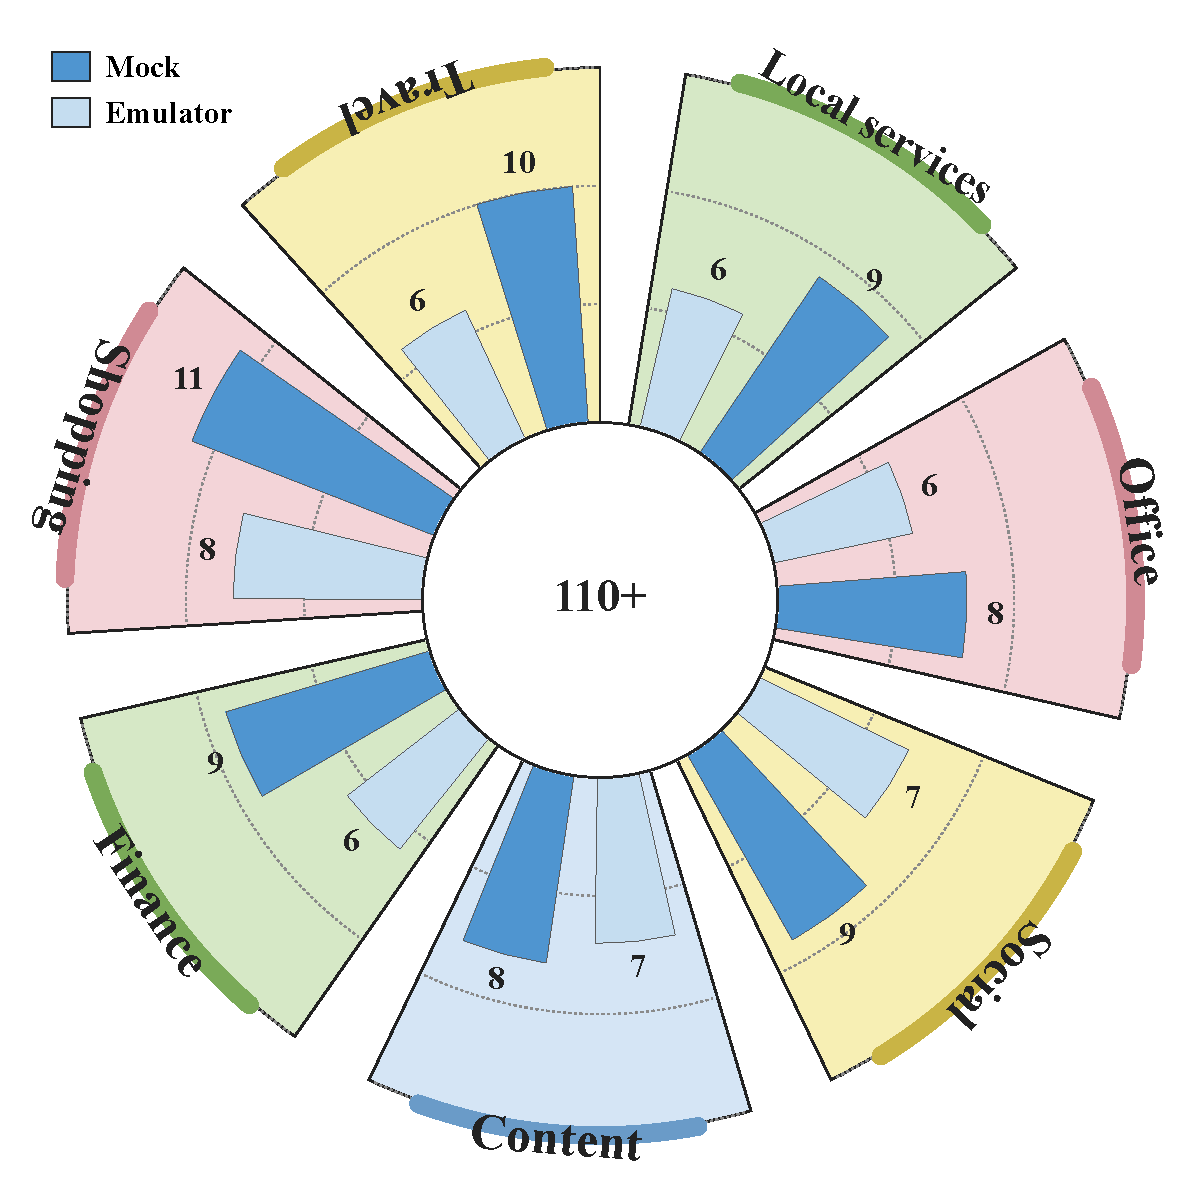
\includegraphics[height=3.9cm]{figures/exp-app-pies.pdf}\\[0.3em]
{\small (a) Application coverage}
\end{minipage}
\hfill
\begin{minipage}[b]{0.68\linewidth}
\centering
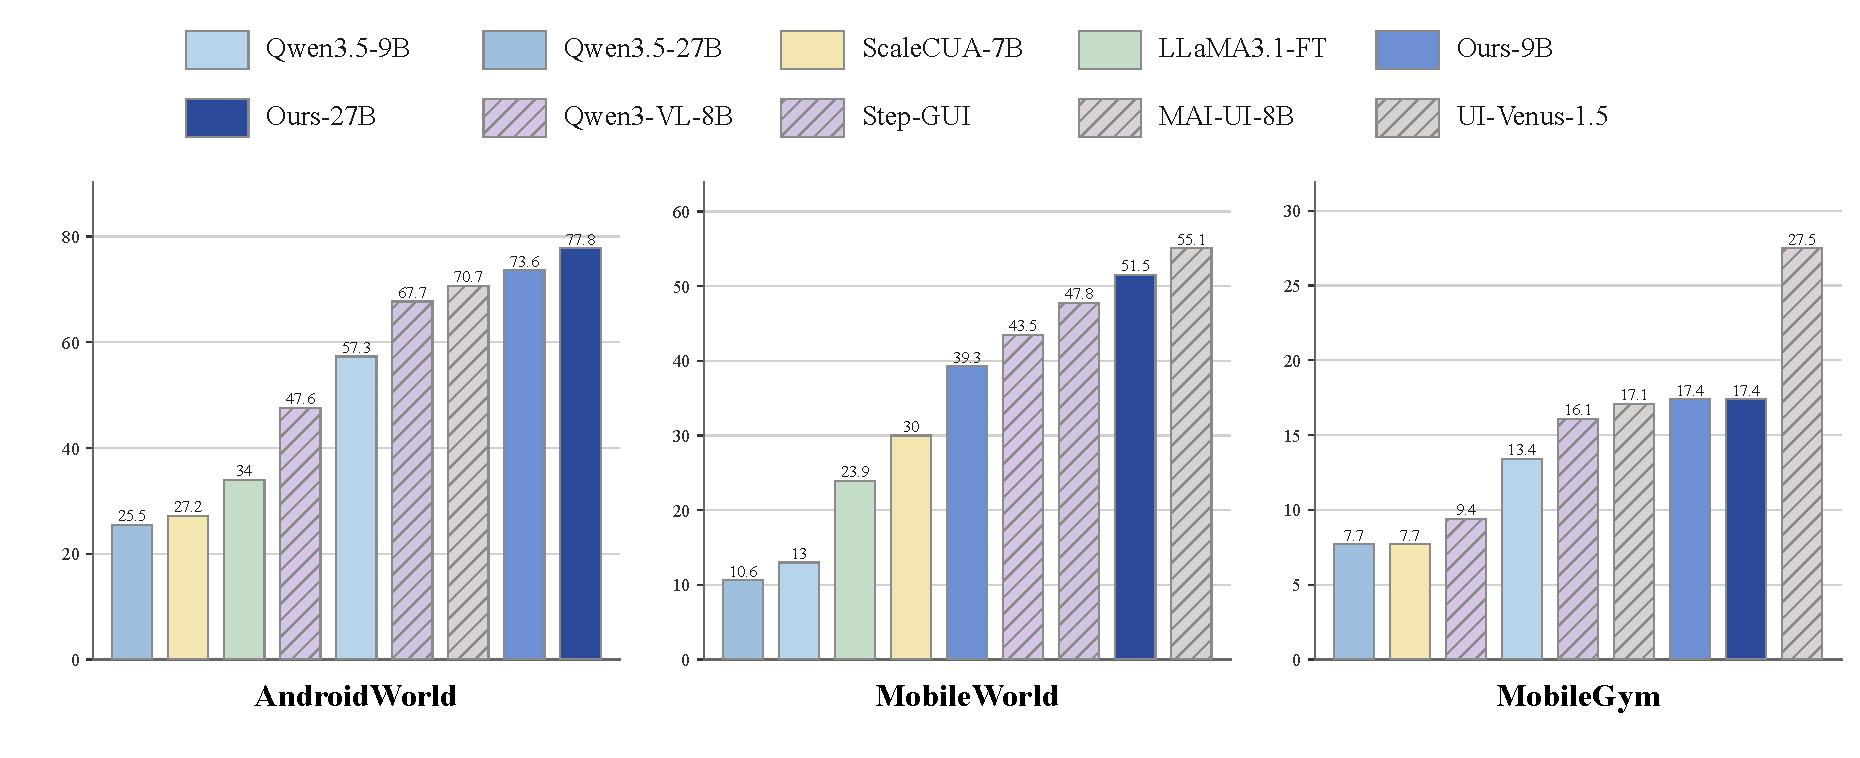
\includegraphics[height=3.9cm]{figures/exp-main-bars.pdf}\\[0.3em]
{\small (b) Benchmark results}
\end{minipage}
\end{center}
\caption{(a)~Application coverage in OpenMobile-V2. Each sector is a functional domain; the two bars are mock (dark) and emulator (light) apps. (b)~Results on AndroidWorld, MobileGym, and MobileWorld.}
\label{fig:intro-overview}
\end{figure}
% Owner: first author
% Scope: OpenMobile-2 --- open agent, diverse environments, training data, hybrid GUI--tool use
\section{Introduction}
\label{sec:intro}

As mobile agents are increasingly expected to handle long-horizon tasks across diverse applications, the scale and breadth of training experience have become critical to their development~\citep{yang2023appagent,wang2024mobileagent,cheng2024seeclick,hong2024cogagent,qin2025uitars,liu2024autoglm,wu2025osatlas}. Scaling such experience requires both broad coverage of applications and workflows and a reliable way to turn interactions into executable learning signals. In particular, an effective training environment should expose agents to diverse mobile experiences while allowing task outcomes to be reset, executed, and verified programmatically.

Existing work has made substantial progress toward these goals, including large-scale interaction datasets~\citep{rawles2023aitw,li2024androidcontrol}, dynamic benchmarks~\citep{rawles2025androidworld,xu2025androidlab,chen2024spabench,kong2025mobileworld}, controllable environments~\citep{wu2026mobilegym}, and open pipelines for task and trajectory generation~\citep{cheng2026openmobile}. Yet existing resources typically trade off breadth of mobile experience against the controllability needed for large-scale training. Realistic applications and workflows are difficult to reset and verify, while controllable environments often cover a narrower range of applications. This makes it difficult to obtain diverse training experience together with executable tasks and reliable rewards, limiting the scale at which mobile agents can be trained with environment feedback.

We introduce \textbf{OpenMobile-2}, an open training and evaluation stack that addresses this gap through a controllable yet diverse mobile environment and executable training tasks (Figure~\ref{fig:intro-overview}). We build \textbf{MobileGym++}, adding 35 commercial-style applications and cross-app workflows while preserving clean resets and programmatic verification. Together with newly configured Android-emulator applications, the playground covers over 110 applications spanning travel, shopping, finance, content, social, office, and local services. On this foundation, we curate 12K mobile interaction trajectories for supervised fine-tuning and more than 2K executable tasks with automatic rewards for reinforcement learning. Beyond the core training setup, we also expose over 300 scoped app-native tools across 50 applications, enabling GUI actions and tool calls to be interleaved within the same task. This extension allows us to study hybrid GUI--tool interaction in MobileGym++ Bench, where GUI-only and hybrid policies are evaluated on the same long-horizon tasks with the same programmatic checkers.

Training with this open stack produces a strong mobile agent that transfers across environments and interaction settings. OpenMobile-2 achieves \textbf{77.8} on AndroidWorld, \textbf{40.2} on MobileWorld, and \textbf{44.7} on MobileGym (Figure~\ref{fig:intro-overview}b), while also transferring to real-device mobile use. These results demonstrate that diverse and verifiable open environments, combined with scalable supervised and executable reinforcement-learning data, can support competitive mobile-agent performance beyond the training playground. More importantly, the unified interface and evaluation framework enables controlled study of GUI-only and hybrid GUI--tool interaction without changing the underlying task or verifier. All environments, data, tools, benchmarks, and training recipes will be open-sourced at XXX.

Our main contributions are:
\begin{itemize}
\item \textbf{A diverse and verifiable mobile-agent playground.} We introduce MobileGym++, extending a controllable mobile runtime with 35 commercial-style applications and cross-app workflows. Together with newly configured emulator applications, the playground covers over 110 applications while retaining clean resets and programmatic verification.
\item \textbf{Open training data for supervised and reinforcement learning.} We release 12K mobile interaction trajectories and more than 2K executable RL tasks with automatic rewards, together with the corresponding training recipes, enabling scalable training from both demonstrations and environment-grounded feedback.

\item \textbf{A unified framework for GUI and native tool use.} We integrate over 300 scoped app-native tools across 50 applications and introduce MobileGym++ Bench, where GUI-only and hybrid GUI--tool agents can be evaluated on the same long-horizon tasks with the same programmatic checkers.
\end{itemize}
% Owner: ________
% Scope: GUI agents, mobile environments, hybrid GUI + native tool use
\section{Related Work}
\label{sec:related}

\paragraph{GUI Agents.}
Early GUI agents operated on structured representations such as HTML, accessibility trees, or view hierarchies. These signals can be long, incomplete, or unavailable on some platforms, motivating purely visual agents that act directly from screenshots~\citep{cheng2024seeclick,hong2024cogagent}. Subsequent work improved GUI grounding and cross-platform action modeling~\citep{wu2025osatlas}, while mobile-specific systems demonstrated that multimodal models can complete multi-step phone tasks through tapping, typing, and swiping~\citep{yang2023appagent,wang2024mobileagent}. More recent foundation agents have further improved mobile task performance through large-scale training and online reinforcement learning~\citep{liu2024autoglm,qin2025uitars}. Despite these advances, the dominant interaction paradigm remains GUI-based: agents perceive pixels, optionally augmented with UI structure, and emit low-level actions. 

\paragraph{Mobile Environments.}
Offline corpora such as AITW and AndroidControl provide large-scale human demonstrations for mobile interaction~\citep{rawles2023aitw,li2024androidcontrol}. Interactive environments have subsequently enabled agents to execute and evaluate tasks directly on Android devices and emulators. AndroidWorld provides a widely used open environment with 116 programmatic tasks across 20 Android applications, featuring parameterized instructions and state-based rewards~\citep{rawles2025androidworld}. AndroidLab and SPA-Bench further expand the range of tasks and application settings, while MobileWorld pushes toward more challenging long-horizon and cross-application workflows and introduces MCP-augmented interaction~\citep{xu2025androidlab,chen2024spabench,kong2025mobileworld}. Complementing these device- and emulator-based environments, MobileGym takes a simulation-based approach by recreating application experiences in a browser-hosted sandbox and mocking external dependencies, enabling commercial-style workflows to be reset, programmatically verified, and rolled out in parallel~\citep{wu2026mobilegym}. Together, these efforts have progressively expanded the scale, diversity, and executability of mobile-agent environments, providing increasingly strong foundations for both training and evaluation.

\paragraph{Hybrid GUI and App-Native Tool Use.}
Beyond low-level GUI actions, recent work has explored richer interfaces for software interaction. On desktop, UFO and UFO$^2$ combine UI automation with application-level APIs, while OS-Copilot exposes heterogeneous capabilities such as bash, Python, and APIs alongside mouse and keyboard interaction~\citep{zhang2024ufo,zhang2025ufo2,wu2024oscopilot}. The Model Context Protocol (MCP) provides a standardized protocol for exposing and invoking tools across applications~\citep{anthropic2024mcp}. In the mobile domain, MobileWorld incorporates MCP-based tool interaction into its evaluation tasks~\citep{kong2025mobileworld}. These approaches extend the action space beyond direct GUI manipulation by allowing agents to invoke structured application or system capabilities. A related setting is to expose selected application functionalities as app-native tools alongside the GUI, allowing GUI actions and tool calls to be interleaved within the same task while retaining the GUI as a complete interaction interface.


% Owner: environment / benchmark (this chapter)
% Do not put 120+ or unofficial run scores here.
% Cross-refs: \ref{sec:intro}, \ref{sec:related}, \ref{sec:exp},
%   \ref{tab:mgpp-compare}, \ref{app:mgpp-apps}, \ref{app:mgpp-tools}
\section{MobileGym++}
\label{sec:mobilegym++}
\label{sec:method}

\subsection{A gap in controllable commercial applications}
\label{sec:mgpp-env}

Mobile agents are moving from system utilities and open-source clients into a larger commercial application world. Travel booking, online shopping, personal finance, and local services occupy most of a user's daily time, and they are the settings agents must eventually enter. Scaling evaluation and training into those settings, however, hits a structural bottleneck on each of the two paths now available.

One path runs real applications on physical devices. It buys interface and network fidelity at the cost of device state that is hard to reset or parallelize. Many commercial apps refuse to load once they detect an automation environment, so collection is pinned to particular devices and accounts, and an order, a payment, or a sent message during an experiment is an irreversible write into the real world. The other path runs reproducible applications in a controllable environment. It buys reset and a deterministic checker at the cost of an inclusion rule that favors offline, login-free software---mostly system utilities and open-source clients. AndroidWorld's rewards come from system state read through debugging interfaces: they can confirm a calendar event or a contact change, but not the amount paid or the recipient on a third-party shopping order~\citep{rawles2025androidworld}. AppWorld supplies a controllable world and state-based programmatic evaluation, but its action space is function calls and there is no operable graphical interface~\citep{trivedi2024appworld}. MobileWorld adds cross-application work and external tools, yet many items are written so that they are hard to finish without those tools~\citep{kong2025mobileworld}. In earlier controllable suites, the terminals a program can check concentrate on system settings and local files. Completing an order, posting an expense, or changing an itinerary still has nowhere stable to land.

Judgment choices shrink the usable range further. A model judge introduces unstable false positives. Once an online site is taken offline, its native verifier no longer applies and comparison falls back to matching a reference trajectory, whose gap from other valid paths is hard to close. For a setting that is meant to serve both academic and industrial use, the check has to land on the application's own business objects---and that is possible only when the application itself is fully controllable.

Neither path, then, carries scalable evaluation and training through a complete commercial operation. The device path cannot reset state or undo side effects; the controllable path is narrow in application mix and shallow in what the terminal proxy can see. Covering commercial work depends on constructing controllable mock commercial applications.

MobileGym++ is the response: a browser-hosted mobile environment that reproduces closed commercial loops. It ships 64 installable applications, 35 of them newly built commercial clients, covering travel, shopping, finance, content, social, office, and local services. Authenticity, diversity, and stability are the acceptance criteria. Authenticity is the closed loop---goods and orders, expenses and budgets, itineraries and changes exist as objects in each app's own store. Diversity is the seven domains and 64 applications. Stability is an initial state that can be exported and restored as a whole, together with a programmatic checker that reads only business state. The runtime is MobileGym~\citep{wu2026mobilegym}. Serialization, reset, inter-app navigation, and programmatic checking are inherited. What this paper expands is the content those mechanisms carry, and one new calling channel.

\subsection{Platform and expansions}
\label{sec:mgpp-inherit}

The predecessor already supplies a complete controllable runtime. The device runs inside a browser tab; each app keeps a structured store and renders its UI from that store; the clipboard, system broadcasts, and inter-app navigation already connect apps; the full device state can be exported as one record and restored from it; many instances can run at once without interfering. On the agent side, observations remain screen pixels. There is no accessibility tree, and the agent cannot read the business store. Actions remain discrete taps, swipes, typing, and navigation; at most one action executes per step.

On that same runtime we make two expansions. The first spreads reproducible commercial clients to a scale that covers domains. Newly built apps reproduce a business loop rather than a skin. Each client is built from a real product: the object model and state transitions are fixed first, then the business functions and pages. Goods and orders, expenses and budgets, itineraries and changes, conversations and messages exist as objects in the app's own store. The UI renders them; the checker reads them. Before admission, each newly built app must pass a page-reachability check and a terminal-state checkability check. The second expansion opens, inside the apps, a set of function calls with the same rights as the GUI; we return to it in Section~\ref{sec:mgpp-tools}.

\subsection{Programmatic checks on business state}
\label{sec:mgpp-check}

A task binds an initial state. At the end we take a diff of the full device state and ask whether the target business fields were written as required. The checker depends on neither a model judge nor a single reference trajectory: different routes that accomplish the same write are equivalent. Programmatic state checking is already shared practice in controllable environments. AppWorld contrasts state-based evaluation with the brittleness of reference matching~\citep{trivedi2024appworld}; AndroidWorld notes that system state outlasts matching surface UI changes~\citep{rawles2025androidworld}; MobileGym states that checks are deterministic, fine-grained, and independent of a vision-language judge~\citep{wu2026mobilegym}. The difference here is not the mechanism but the object being read. The checker reads the app's own business store, so a commercial result can enter evaluation. Treating a system setting or a widget tree as a terminal proxy cannot cover an operation whose landing point is a business object.

Checks are written as relations, not as constants. An expense amount must equal the payment that just completed; a calendar title must contain the selected train number. Constants appear only in the initial state. Outside the target fields, a task declares which state paths may change; remaining diffs are recorded as unexpected mutations and reported separately from success. A task counts as cross-application if and only if the checker reads a business write in at least two apps. Querying and then paraphrasing, or sending a notification into a second app, does not count.

\subsection{Scale, depth, and coverage}
\label{sec:mgpp-scale}

The environment ships 64 installable applications, 35 of them newly built commercial clients, organized by the seven domains above. Each domain carries a different object type and a different terminal form---placing an order, posting a ledger entry, creating an itinerary, sending a message, adding a favorite---so the same checker template cannot cover them all.

Count alone is not enough; each app must be deep enough to carry a multi-step task. On the newly built clients, the median navigation declaration is 37 routes, 175 interactive actions, and 88 transitions. As a depth reference, the thickest application in MobileGym has 100 routes and 265 actions, and its deepest terminal takes 7 steps to reach. Median interaction depth from the root in this environment is 3: the shortest GUI path of a typical task already crosses several layers, and the step-count lower bound comes from page structure rather than from the length of the instruction. Table~\ref{tab:mgpp-compare} summarizes how this environment differs from other controllable gyms in what a program is allowed to read. Per-app statistics are in Appendix~\ref{app:mgpp-apps}.

\begin{table}[t]
\caption{Controllable environments. The checker column is what a program is allowed to read; the tool column is whether a call writes the same store as the GUI. Real-device gyms are omitted: they cover vendor apps and live networks, not a resettable commercial store.}
\label{tab:mgpp-compare}
\begin{center}
\scriptsize
\setlength{\tabcolsep}{3pt}
\begin{tabular}{lcccc}
\hline
 & Apps & Checker reads & Cross-app & Tools vs.\ GUI \\
\hline
AndroidWorld & system / default & system state & limited & --- \\
AppWorld & APIs, no phone GUI & application DBs & yes & API only \\
MobileWorld & longer vendor-style & mixed & yes & external MCP \\
MobileGym & mock daily / system & device state diff & OS-level & none \\
MobileGym++ & 64 mock commercial & app business store & dual writes & same store \\
\hline
\end{tabular}
\end{center}
\end{table}

\subsection{In-app tools}
\label{sec:mgpp-tools}

Agents already call functions. Existing evaluation splits that fact across two settings. Graphical environments almost only score taps and typing; interface-only environments have nothing to tap. The behavior that then has nowhere to be tested is the choice itself: when to use the GUI, when to call an interface, and how to return to the screen to confirm. As an extension for future evaluation, this environment places both channels on the same business store, in one runtime. GUI-only research remains valid; no official task path can be finished only through tools.

Approximately 52 applications expose a function interface under their own namespace. The agent may list and call the foreground app's functions. A call occupies the same action slot as a GUI action; at most one of the two executes per step. Those functions act on the app's own store and go through the same business functions as the GUI, so they are a second channel in one world rather than an external service that bypasses the screen. The operations they cover are a strict subset of what the GUI can already finish. Payment confirmation, password entry, and contact picking remain GUI-only. Prefill calls produce a draft and no business write; saving still requires the screen.

A typical mixed solution looks like this. The agent calls the bookkeeping app to read the currently available budget categories, switches to the shopping app, picks an item and completes payment on screen, then calls the bookkeeping app again to write that expense into a named ledger. Payment cannot be finished by a call, because the PIN pad exists only in the GUI. Bookkeeping admits both routes: a save on screen and a function call produce the same record. The checker reads the same fields in either case, and therefore does not distinguish whether the expense was tapped or invoked. Every official task keeps a GUI-only path. A GUI-only solution and a mixed solution are compared on the same task, the same initial state, and the same checker. Protocol and the tool catalog are in Appendix~\ref{app:mgpp-tools}.

\subsection{Benchmark}
\label{sec:mgpp-bench}

\paragraph{Task design.}
Single-app GUI operation is already scored thoroughly. From AndroidWorld to MobileWorld, the typical task is a sequence of interface actions inside one application, and the terminal lands on system-level state or a surface attribute of the app---editing a contact, toggling a setting, creating a calendar event~\citep{rawles2025androidworld,kong2025mobileworld}. Along that axis, existing coverage reduces to an in-app interface chain whose terminal is proxied by system state or a widget tree. That axis is densely and maturely scored. It does not reach two further places.

The first is a business write as the terminal. Completing an order, posting an expense, or changing an itinerary does not land in a system setting or on a widget tree; it lands in the app's own business store. On the real-device path, that store cannot be read in full by an external program, so checking falls back to screenshot matching or a model judge. On the controllable path, earlier environments stop at system utilities and open-source clients, and the business store itself is absent. Operations whose landing point is a business object therefore still lack a programmatic terminal.

The second is a cross-application value dependence. In a single-app task, everything needed to finish is usually written in the instruction or already visible on the current screen. In a commercial process, the number a write needs often comes from another app's live state: the amount actually paid after checkout must be posted to a ledger; the selected train must be copied into a calendar. The agent must read the value in one app and write it into the correct field in another. Cross-application items in existing suites mostly stop at querying and then paraphrasing, or at sending a notification; the second app does not produce a business write that depends on a fact from the first, and no checker can ask whether the two apps' fields line up.

MobileGym++ Bench sits on the environment above and occupies exactly those two extensions. Every task ends in a business write that actually occurs. Tasks that only query, only open a page, or only restate a result in text do not enter the official set. Realism comes from the process, not from the wording of the prompt: a task is long because it must pass through selection, confirmation, payment, and write-back, not because unrelated steps were stacked. The instruction is written as a user would speak it; it does not name widget labels, in-app namespace identifiers, or checker fields.

In a cross-application task the needed number is absent from the instruction and present in another app's live store. The instruction gives a pointer---``the amount actually paid'', ``the largest charge'', ``this train''---and the checker asks whether the two apps' fields line up, not whether a constant written in advance appears. The relation moves with the environment state and cannot be solved by memorizing constants in the prompt.

A GUI-only solution is a first-class citizen. Every task keeps at least one GUI-only path; a mixed solution is another path in the same world, reported under the same checker.

Difficulty does not come from a longer prompt or from stacked unrelated steps. It comes from the structural cost of finishing a write. Median shortest GUI path in the environment is 3; deeper tasks enter further layers, and that lower bound is set by page structure. The same business action can look finished on screen and land in different store fields: ledger category, order ownership, and message channel are distinct. The checker reads the field; stopping on a result page is not evidence of completion. A cross-application task additionally requires the agent to read the needed value in one app and write it in another, and both stores are read by the checker.

\paragraph{Task specification.}
Each task has three published parts: a natural-language user goal, a bound initial state, and a programmatic check on the terminal state. The checker reads the before/after diff of business state. It does not read the trace, does not read screenshots, and does not accept an agent's claim of completion. Paths that the task allows to change are declared; other diffs are reported as unexpected mutations, separately from success.

\paragraph{Scale and composition.}
Tasks are organized by business domain, not by application, and cover the same seven domains as the environment. The design size is approximately 200 tasks, of which approximately 116 are single-app and 84 are cross-application under the write-based definition above. Each frequently used app carries several tasks, and a few high-frequency apps carry more, so that evaluation is not dominated by a handful of apps and no app is covered by a single item. Only tasks that meet the checker-level definition count as cross-application---a business write in at least two apps. An app that appears only as a notification channel is not counted toward its domain's cross-application coverage.

\paragraph{Evaluation protocol.}
The primary metric is task success rate. Step counts are reported on successful tasks as an efficiency reference; failed trajectories often stop before the step cap, and those steps are excluded from the efficiency statistic. The main table reports two success rates on the same tasks, the same initial state, and the same checker: GUI-only and mixed. They have equal status. The release includes the task definitions, the initial-state records, and the read paths the checker uses. Runtime version and the time base used in evaluation are locked in the protocol so that runs remain comparable.

% Owner: ________
% Scope: setup, baselines, main results, ablations, analysis
% Tables and figures for this section live in figures/ with labels prefixed by exp-.
\section{Experiments}
\label{sec:exp}

TODO: Write the experiments.

% \subsection{Experimental setup}
% \label{sec:exp-setup}
%
% \subsection{Main results}
% \label{sec:exp-main}
%
% \begin{table}[t]
% \caption{Main comparison. Best results are in bold.}
% \label{tab:exp-main}
% \begin{center}
% \begin{tabular}{lcc}
% \multicolumn{1}{c}{\bf Method} & \multicolumn{1}{c}{\bf Metric A} & \multicolumn{1}{c}{\bf Metric B} \\
% \hline
% Baseline & -- & -- \\
% Ours     & -- & -- \\
% \end{tabular}
% \end{center}
% \end{table}
%
% \subsection{Ablations}
% \label{sec:exp-ablation}

% Owner: ________
% Scope: summary of findings, limitations, future work
% Keep this short; ICLR main text is 9 pages (10 camera-ready).
\section{Conclusion}
\label{sec:conclusion}

TODO: Write the conclusion.


% Required / recommended statements: do not count toward the page limit.
% Owner: corresponding author (collect input from everyone)
% Required. Does not count toward the page limit. At most 1 page.
\subsection*{AI use statement}

TODO: Follow the ICLR 2027 AI Policy for Authors.

In this work, we used generative AI tools for [tasks with required disclosure].
We have not used generative AI tools for [other tasks with required disclosure],
and [the rest of the required disclosure tasks] are not applicable to this work.
Additionally, we used generative AI tools for [tasks with recommended
disclosure]. We have reviewed all AI-assisted work. We take responsibility for
the final content of this work, including text, claims or artifacts produced
with the aid of generative AI.

% Owner: ________
% Recommended. Does not count toward the page limit. At most 1 page.
\subsection*{Ethics statement}

TODO: If this work raises ethics issues (human subjects, data release, dual use,
bias, privacy, legal compliance, research integrity), address them here.
Otherwise keep a short statement that no such issues apply.

% Owner: experiments lead
% Recommended. Does not count toward the page limit.
% Point to code, appendix proofs, and data-processing details; do not dump them here.
\subsection*{Reproducibility statement}

TODO: Point to the anonymous code, the appendix sections that contain proofs or
hyperparameters, and any dataset processing steps needed to reproduce the results.
See Section~\ref{sec:exp} and Appendix~\ref{app:details}.


\subsubsection*{Author Contributions}
% Optional. Fill in before camera-ready if desired.
Author One led Section~\ref{sec:intro}.
Author Two led Section~\ref{sec:method}.
Author Three led Section~\ref{sec:exp}.

\subsubsection*{Acknowledgments}
Use unnumbered third-level headings for acknowledgments. Funding acknowledgements go here, not in author footnotes.

\bibliography{iclr2027_conference}
\bibliographystyle{iclr2027_conference}

\appendix
% Owner: method + experiments leads (split with \section if needed)
% Unlimited pages. Put proofs, extra ablations, hyperparameters, dataset details here.
\section{Additional Details}
\label{app:details}

TODO: Appendix material.

% If two people share the appendix, split into extra files and \input them
% from this file or from main.tex after \appendix, e.g.:
%   chapters/A1_proofs.tex
%   chapters/A2_extra_exps.tex


\end{document}
